\documentclass[12pt]{article}

%%%%%%%%%%%%%%%%%%%%%%%%%%%%%%%%%%%%%%%%%%%%%%%%%%%%%%%%%%%%%%%%%%%%%%%%%%%%%%%%%%%%%%%%%%%
%                                     Page Numbers
%%%%%%%%%%%%%%%%%%%%%%%%%%%%%%%%%%%%%%%%%%%%%%%%%%%%%%%%%%%%%%%%%%%%%%%%%%%%%%%%%%%%%%%%%%%

\usepackage{fancyhdr}
\fancyhf{}
\fancyfoot[C]{\thepage}
\renewcommand{\headrulewidth}{0pt}
\renewcommand{\footrulewidth}{0pt}
\pagestyle{plain}

%%%%%%%%%%%%%%%%%%%%%%%%%%%%%%%%%%%%%%%%%%%%%%%%%%%%%%%%%%%%%%%%%%%%%%%%%%%%%%%%%%%%%%%%%%%
%                                     Imports
%%%%%%%%%%%%%%%%%%%%%%%%%%%%%%%%%%%%%%%%%%%%%%%%%%%%%%%%%%%%%%%%%%%%%%%%%%%%%%%%%%%%%%%%%%%

\usepackage{aaspp4}
\usepackage{epsf}
\usepackage{flushrt}
\usepackage{textpos}
\usepackage{graphicx}
\usepackage{listings}
\usepackage{color}
\usepackage{colortbl}
\usepackage{hyperref}
\usepackage{float}
\usepackage{indentfirst}
\usepackage{subfigure}
\usepackage[format=plain, labelsep=none, justification=justified, font=footnotesize, labelfont=it, singlelinecheck=false]{caption}

%%%%%%%%%%%%%%%%%%%%%%%%%%%%%%%%%%%%%%%%%%%%%%%%%%%%%%%%%%%%%%%%%%%%%%%%%%%%%%%%%%%%%%%%%%%
%                                     My additions
%%%%%%%%%%%%%%%%%%%%%%%%%%%%%%%%%%%%%%%%%%%%%%%%%%%%%%%%%%%%%%%%%%%%%%%%%%%%%%%%%%%%%%%%%%%

% colors
\usepackage{color}
\definecolor{dkgreen}{rgb}{0,0.6,0}
\definecolor{gray}{rgb}{0.5,0.5,.5}
\definecolor{mauve}{rgb}{0.58,0,0.82}
\definecolor{lgray}{rgb}{0.9,0.9,0.9}


% code settings
\usepackage{listings}
\lstset{frame=tb,
    language=Python,
    aboveskip=3mm,
    belowskip=3mm,
    showstringspaces=false,
    columns=flexible,
    basicstyle={\small\ttfamily},
    numbers=none,
    numberstyle=\tiny\color{gray},
    keywordstyle=\color{blue},
    commentstyle=\color{dkgreen},
    stringstyle=\color{mauve},
    backgroundcolor=\color{lgray},
    % morestring=[s]{`}{'},
    % morestring=[s]{``}{''},
    breaklines=true,
    breakatwhitespace=true,
    tabsize=3
}

%%%%%%%%%%%%%%%%%%%%%%%%%%%%%%%%%%%%%%%%%%%%%%%%%%%%%%%%%%%%%%%%%%%%%%%%%%%%%%%%%%%%%%%%%%%
%                                User definitions
%%%%%%%%%%%%%%%%%%%%%%%%%%%%%%%%%%%%%%%%%%%%%%%%%%%%%%%%%%%%%%%%%%%%%%%%%%%%%%%%%%%%%%%%%%%

\pagestyle{fancy}
\pagenumbering{arabic}

% Page size and margins
\usepackage{geometry}
\geometry{letterpaper, portrait, margin=1in}

% Sections
% \def\ssection#1{\section{\hbox to \hsize{\large\bf #1\hfill}}}
% \def\ssectionstar#1{\section*{\hbox to \hsize{\large\bf #1\hfill}}}

% References
\newenvironment{pgrefs}{\bigskip
   \begin{flushleft} {\large \bf References} \end{flushleft} \bigskip
   \medskip
   \begin{list}{}{\setlength{\leftmargin}{1cm}\setlength{\itemindent}{-1cm}
   \setlength{\topsep}{0cm}\setlength{\itemsep}{-0.12cm}}
   \vspace*{-0.6cm}}{\end{list}}

% Footnote
\long\def\symbolfootnote[#1]#2{\begingroup%
  \def\thefootnote{\fnsymbol{footnote}}\footnote[#1]{#2}\endgroup%
  \def\footnoterule{\null}}

% Colors
\definecolor{gray}{gray}{0.85}


%%%%%%%%%%%%%%%%%%%%%%%%%%%%%%%%%%%%%%%%%%%%%%%%%%%%%%%%%%%%%%%%%%%%%%%%%%%%%%%%%%%%%%%%%%%
%                                Title and authors
%%%%%%%%%%%%%%%%%%%%%%%%%%%%%%%%%%%%%%%%%%%%%%%%%%%%%%%%%%%%%%%%%%%%%%%%%%%%%%%%%%%%%%%%%%%

\begin{document}

% Logo
\begin{figure*}[h]
\begin{minipage}[t]{40cm}

\includegraphics[height=35mm]{images/stlogo.png}
\end{minipage}
\end{figure*}

% ISR Number
\begin{flushright}
\vskip -1.3truecm
{\bf Instrument Science Report WFC3 2018-??}
\end{flushright}

% Title and authors
\begin{flushright}
{\huge\bf \hfill Throughput Updates to the WFC3/IR Grism Configuration Files }
\rule{145mm}{0.3mm}
\smallskip \\
    \hfill {G. Brammer \& J. Fowler}\\
 \today
 \end{flushright}
 \medskip

T
%%%%%%%%%%%%%%%%%%%%%%%%%%%%%%%%%%%%%%%%%%%%%%%%%%%%%%%%%%%%%%%%%%%%%%%%%%%%%%%%%%%%%%%%%%%
%                                      Abstract
%%%%%%%%%%%%%%%%%%%%%%%%%%%%%%%%%%%%%%%%%%%%%%%%%%%%%%%%%%%%%%%%%%%%%%%%%%%%%%%%%%%%%%%%%%%

\hrule height 1.5pt
\smallskip
\noindent \large{\bf A}\footnotesize{\bf BSTRACT}

\noindent
\textit{We reduce 7 years of WFC3/IR calibration data on the two 
standard stars GD-71 and GD-153 with the grism reduction software \texttt{grizli}. 
We compare the extracted spectra to preexisting spectroscopy data from the 
\textsc{X-Shooter Spectral Library} (Chen et al, 2014). We analyze ratios of flux profiles 
with wavelength and sensitivity curves to compare with our configuration files
and existing models, look for any calibration difference across detector area,
and look at the calibration of higher order grism fringes.  
We find required changes on the order of ... }

\smallskip
\medskip
\hrule height 1.5pt

\symbolfootnote[0]{Copyright {\copyright} 2016 The Association of
  Universities for Research in Astronomy, Inc. All Rights Reserved.}

%%%%%%%%%%%%%%%%%%%%%%%%%%%%%%%%%%%%%%%%%%%%%%%%%%%%%%%%%%%%%%%%%%%%%%%%%%%%%%%%%%%%%%%%%%%
%                                   Introduction
%%%%%%%%%%%%%%%%%%%%%%%%%%%%%%%%%%%%%%%%%%%%%%%%%%%%%%%%%%%%%%%%%%%%%%%%%%%%%%%%%%%%%%%%%%%

\section{Introduction}

WFC3 (Wide Field Camera 3) of HST (Hubble Space Telescope) has three grisms (spectral elements combining a grating and prism 
to conduct slitless spectroscopy) for the UVIS (UV and visual) and IR
(infrared) channels. For the IR grisms, filters 
G102 and G141, much work has gone into precisely calibrating their wavelength trace and throughput (Pirzkal et. al 2016). 
Recently \texttt{grizli} -- an open source reduction software (Brammer?) was created to extract grism observations 
and provide high quality WFC3/IR and JWST data. 

For this project we extract WFC3/IR grism
observations of GD-71 and GD-153 and compare the WFC3 slitless spectroscopy to the exisiting spectroscopy
both from STIS (the Space Telescope Imaging Spectrograph) and the
\textsc{X-Shooter Spectral Library}. We take care
to not only examine the first order fringes of the grism used for the bulk of science data, but to also 
extract second and negative first order grism fringes. (The distinction is shown in Figure \ref{fig:grism_orders}.)

%fig%%%%-------------------------------------------------------%%%%%%
\begin{figure}[h!]
\makebox[\textwidth][c]{
\mbox{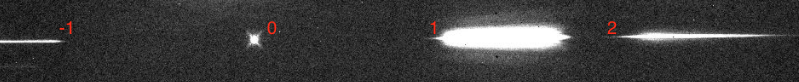
\includegraphics[width=\textwidth]{images/grism_orders.png}}
}
\caption{\textit{An example of a grism observation and the fringe orders. This image is of
    GSC $02581-02323$ in the G14 filter. As numbered, 
    the zeroeth order is what's left in the image of the original source. The first order is
    the brightest projection and the one used predominately for science. The second and negative first 
    order are much fainter (often only visual for bright stars).}}
\label{fig:grism_orders}
\end{figure}
%fig%%%%-------------------------------------------------------%%%%%%


%%%%%%%%%%%%%%%%%%%%%%%%%%%%%%%%%%%%%%%%%%%%%%%%%%%%%%%%%%%%%%%%%%%%%%%%%%%%%%%%%%%%%%%%%%%
%                                       Data
%%%%%%%%%%%%%%%%%%%%%%%%%%%%%%%%%%%%%%%%%%%%%%%%%%%%%%%%%%%%%%%%%%%%%%%%%%%%%%%%%%%%%%%%%%%

\section{Data}

    We began with two WFC3/IR grism data sets on standard calibrator stars
    \href{http://archive.stsci.edu/hst/search.php?action=Search&sci_instrume=WFC3&sci_targname=GD-71&sci_pep_id=11552,11926,11936,12333,12357,12702,13092,13579,14024,14386&sci_aper_1234=IR,G*}{
        \color{blue} GD-71} and
    \href{http://archive.stsci.edu/hst/search.php?action=Search&sci_instrume=WFC3&sci_targname=GD-153&sci_pep_id=11552,11926,11936,12333,12357,12702,13092,13579,14024,14386&sci_aper_1234=IR,G*}{
        \color{blue} GD-153} from the 
Barbara Mikulski Archive for Space Telescopes (MAST); both queries are linked. Each set of 
data includes grism exposures (G102 and G141) and corresponding direct exposures (F105, F098, and F140, F160), 
dithered across the field of view. Grism observations are traditionally taken
in these pairs so the direct image can be used to match the trace (or spatial
extent) to the central source. The data spans 7 years of WFC3/IR grism calibration proposals and consists of 
591 individual exposures (303 for GD-71 and 282 for GD-153). Tables \ref{tab:gd_71} and \ref{tab:gd_153} list the proposals and visits
used for GD-71 and GD-153 respectively. 

%tab%%%%-------------------------------------------------------%%%%%%
\begin{table}[^b]
\makebox[\textwidth][c]{
\begin{tabular}{|l|l|l|l|l|l|l|}
\hline
		Root & Proposal & Visit & PA $^\circ$ & Exposures & Filters & Obs. Date  \\  
\hline
\rowcolor{gray} ibbt & 11936 & 01 & 90.08  & 30 & F098M, F105W, G102                   & 2009-10-03 \\ 
    		     &       & 02 & 89.22  & 30 & F160W, F140W, G141                   & 2009-09-21 \\ 
\rowcolor{gray}      &       & 03 & 274.53 & 30 & F098M, F105W, G102                   & 2010-04-24 \\ 
		     &       & 04 & 275.16 & 30 & F160W, F140W, G141                   & 2010-04-24 \\
\rowcolor{gray} ibcf & 11926 & 04 & 91.08  & 5  & F140W, G141, +$^{*}$                 & 2009-10-05 \\
		     &       & 05 & 90.56  & 5  & F140W, G141, +                       & 2010-02-16 \\
\rowcolor{gray}      &       & 06 & 264.73 & 5  & F140W, G141, +                       & 2010-02-16 \\
		     &       & 29 & 95.73  & 5  & F140W, G141, +                       & 2009-11-01 \\
\rowcolor{gray}      &       & 30 & 104.62 & 5  & F140W, G141, +                       & 2009-11-25 \\
		iblf & 12357 & 01 & 235.00 & 30 & F098M, F105W, G102                   & 2011-01-14 \\
\rowcolor{gray}      &       & 02 & 209.57 & 30 & F160W, F140W, G141                   & 2010-12-24 \\
		ibll & 12333 & 14 & 105.00 & 14 & F098M, G102, F140W, G141             & 2010-11-17 \\
\rowcolor{gray} ibwq & 12702 & 02 & 235.00 & 12 & F098M, F105W, G102, F160, F140, G141 & 2011-12-31 \\
		icqw & 14024 & 01 & 265.74 & 36 & F098M, F105W, G102                   & 2015-01-02 \\
\rowcolor{gray}      &       & 02 & 265.74 & 36 & F160W, F140M, G141                   & 2015-02-08 \\
\hline
\end{tabular}
} 
\caption{\textsl{The above data (303 exposures) make up the body of data used for the GD-71 analysis. These
    exposures consist of grism observations (in G102 and G141) and the accompanying direct exposures
    in F105W or F098M for G102 and F140W and F160W for G141. The + indicates exposures with more filters were taken in the visit, but 
    are not relevant to grism analysis. Note these visits and proposals consist of WFC3 grism calibration proposals.}}
\label{tab:gd_71}
\end{table}
%tab%%%%-------------------------------------------------------%%%%%%

%tab%%%%-------------------------------------------------------%%%%%%
\begin{table}[h!]
\makebox[\textwidth][c]{
\begin{tabular}{|l|l|l|l|l|l|l|}
\hline
		Root & Proposal & Visit & PA $^\circ$ & Exposures & Filters & Obs. Date  \\  
\rowcolor{gray} iab9 & 11552 & 01 & 277.04 & 9  & F098M, F105W, G102                   & 2009-09-09 \\ 
		     &       & 04 & 276.20 & 9  & F160W, F140W, G141                   & 2009-09-09 \\ 
\rowcolor{gray}      &	     & A1 & 291.37 & 3  & F098M, F105W, G102                   & 2009-09-09 \\ 
		     &       & A4 & 291.36 & 3  & F160W, F140W, G141                   & 2009-09-09 \\
\rowcolor{gray} ibwq & 12702 & 1A & 291.37 & 48 & F098M, F105W, G102                   & 2012-06-23 \\
		     &       & 1B & 291.37 & 42 & F160W, F140W, G141                   & 2012-05-18 \\
\rowcolor{gray}      &       & AA & 292.14 & 9  & F098M, F105W, G102, F160, F140, G141 & 2012-06-24 \\
		     &       & AB & 292.15 & 3  & F160W, F140W, G141                   & 2012-05-18 \\
\rowcolor{gray} ic46 & 13092 & 1A & 292.14 & 28 & F098M, F105W, G102, F160, F140, G141 & 2013-06-01 \\
		ich4 & 13579 & 01 & 292.00 & 28 & F098M, F105W, G102, F160, F140, G141 & 2014-06-24 \\
\rowcolor{gray}      &       & 02 & 292.00 & 28 & F098M, F105W, G102, F160, F140, G141 & 2014-07-05 \\
		id2q & 14386 & 01 & 326.00 & 36 & F098M, G102, F140W, G141             & 2016-05-02 \\
\rowcolor{gray}      &       & 02 & 346.24 & 36 & F160W, F140W, G141                   & 2016-04-13 \\
\hline
\end{tabular}
} 
\caption{\textsl{The above data (282 exposures) make up the body of data used for the GD-153 analysis.}}
\label{tab:gd_153}
\end{table}
%tab%%%%-------------------------------------------------------%%%%%%

The data on each calibrator was dithered across the detector
to provide a track on how (if at all) the extraction varied with detector
position (which has been true of the WFC3/UVIS grism, as described in Pirzkal et
al. 2017). Figure
\ref{fig:detector_pos} shows the detector position (as calculated by \texttt{astropy.wcs}) 
for the grism observations of both calibrator stars. Downloadable CSV
files that list the RA/DEC, detector position, rootname, proposal ID, and
filter are available ... somewhere.

%fig%%%%-------------------------------------------------------%%%%%%
\begin{figure}[h!]
\makebox[\textwidth][c]{
    \mbox{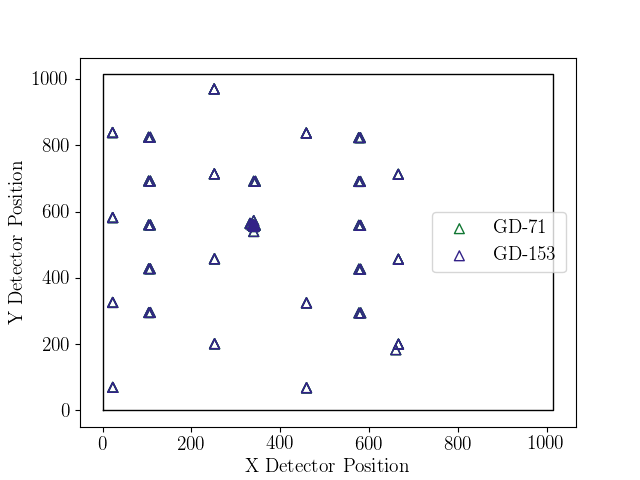
\includegraphics[width=.8\textwidth]{images/dither_grism.png}
    }}
	\caption{\textit{The detector position of the target source (GD-71 or
        GD-153 in blue and green respectively) taken by the grism. Note there
        is little difference in the detector position between the two standard
        stars. 
        Most of the detector area is covered by the dithering and our results
        show no detector position dependence.}}
\label{fig:detector_pos}
\end{figure}
%fig%%%%-------------------------------------------------------%%%%%%

\section{Spectral Extraction with \texttt{grizli}}

The data were reduced using the grism reduction software \texttt{grizli}. Thus far, grizli 
has been predominately used for more compact (and generally single-epoch) datasets. The details of the
extraction are beyond the scope of this ISR, but documented in detail in a 
\href{http://grizli-calibration.readthedocs.io/en/latest/}{\color{blue} \texttt{grizli} cookbook}.

In summary, the grism extraction and analysis required : 
\begin{itemize}
\item Matching visits by WCS orient and creating direct/grism filter pairs.
    \href{http://grizli-calibration.readthedocs.io/en/latest/visit_matching.html#visit-matching-tools}{
        \color{blue}$\rightarrow$}
\item Preprocessing and drizzling the calibrated FLT files. 
    \href{http://grizli-calibration.readthedocs.io/en/latest/visit_matching.html#actually-matching-and-preprocessing-visits}{
        \color{blue}$\rightarrow$}
\item Creating a drizzled mosaic and a segmentation map of all of the data on each source.
    \href{http://grizli-calibration.readthedocs.io/en/latest/drizzling_extracting_etc.html}{
        \color{blue}$\rightarrow$ }
\item Correcting the segmentation map for proper motion of the main source (as the data spans multiple epochs).
    \href{http://grizli-calibration.readthedocs.io/en/latest/drizzling_extracting_etc.html#correcting-seg-map-for-proper-motion}{
        \color{blue}$\rightarrow$ }
\item Resetting Data Quality flags that flag out grism traces.
    \href{http://grizli-calibration.readthedocs.io/en/latest/objects_models_outputs.html#stopping-the-runaway-dq-flag-train}{
        \color{blue}$\rightarrow$ }
\item Extracting beams and making model comparisons. 
    \href{http://grizli-calibration.readthedocs.io/en/latest/objects_models_outputs.html#beams-and-initial-testing}{
        \color{blue}$\rightarrow$ }
\end{itemize}

\subsection{Products of Grism Extraction} 

\texttt{grizli} utilizes \texttt{Astrodrizzle} to align mulitple direct
observations within a grism data set into one mosaic image. For every direct filter we created drizzled mosaics
of the entirety of each dithered field, shown in Figure \ref{fig:mosaics}. These mosaics allow for the creation 
of segmentation maps (or images that isolate the position of source in the
mosaic) with \texttt{SExtractor} and make any proper motion of the sources evident. 


%fig%%%%-------------------------------------------------------%%%%%%
\begin{figure}[h!]
\makebox[\textwidth][c]{
    \mbox{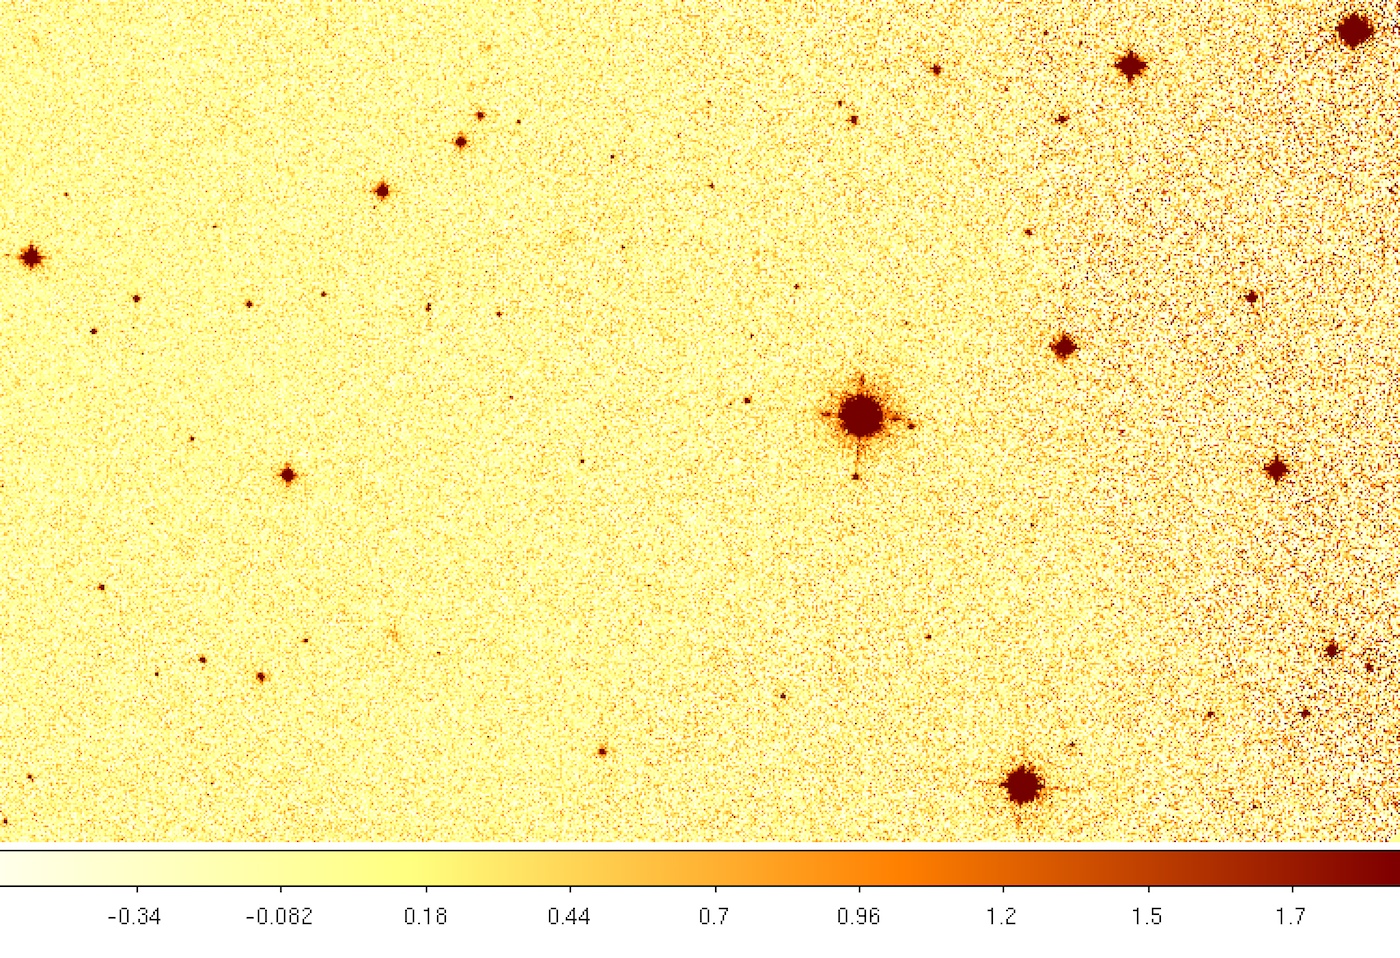
\includegraphics[width=.51\textwidth]{images/drizzled_mosaic-gd71-f105.png}
    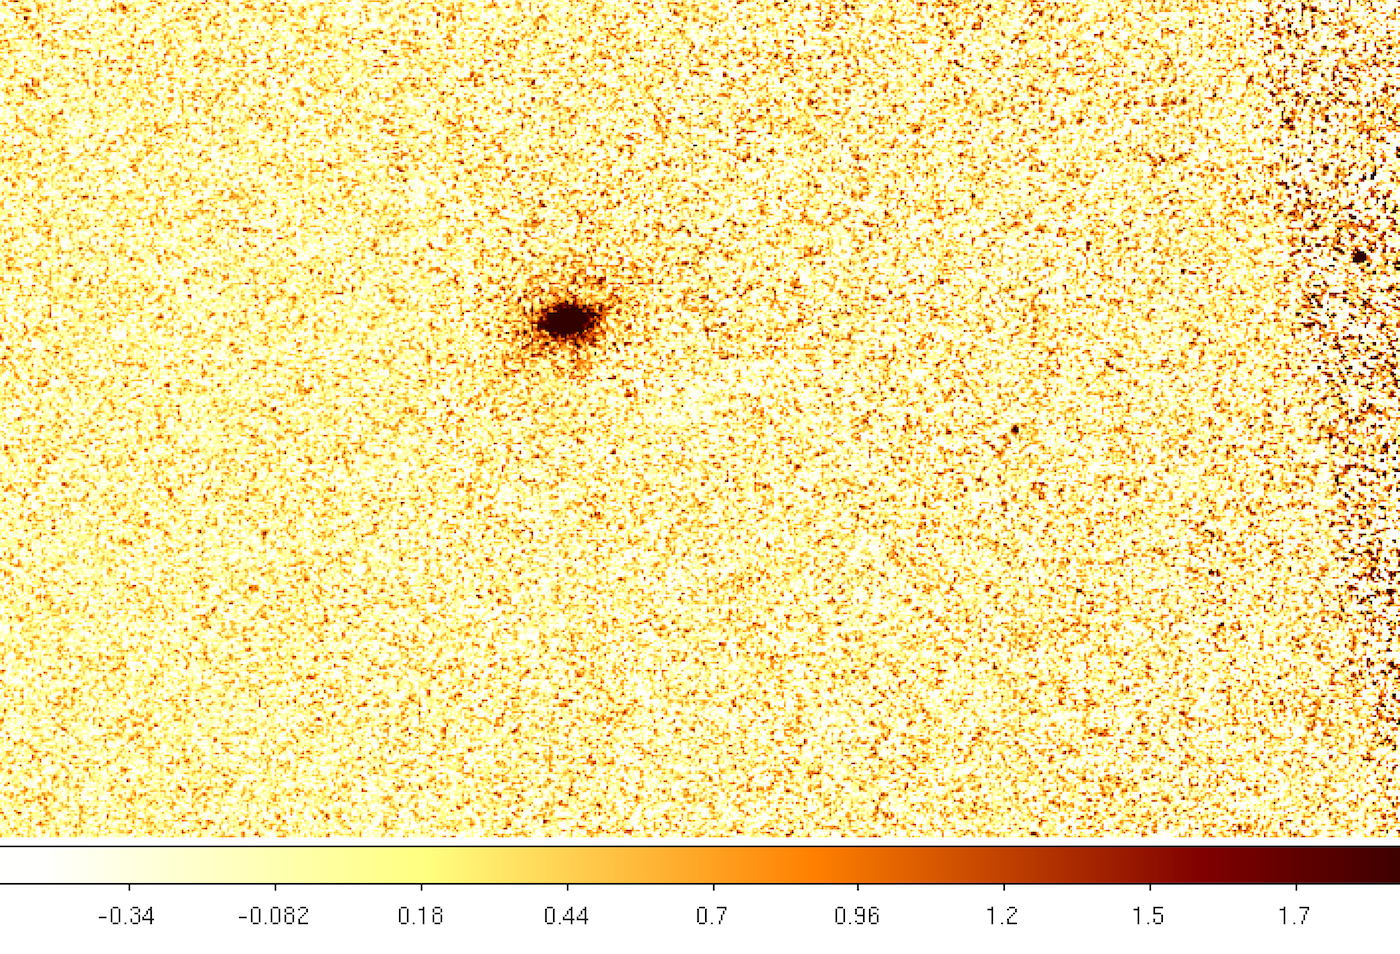
\includegraphics[width=.51\textwidth]{images/proper-motion-source-gd153-f105.png}
    }}
\caption{\textit{Left: An example of a drizzled mosaic image for the dithered field around GD-71 through the F105W.
    Right: A close up of a source artificially extended by proper motion from the field around GD-153 through F105W. 
    (Scale is consistent between the two images.)}}
\label{fig:mosaics}
\end{figure}
%fig%%%%-------------------------------------------------------%%%%%%

We used \texttt{grizli} to create cutouts around each spectral order (or beam) for the standard star. The
beam cutouts allow for closer inspection of the match between the extraction
and model. It is common for Data Quality flags (associated flags to track bad
pixels, cosmic rays, etc) to accidentally flag grisms, and these beam cutouts
make obvious if Data Quality flags have indeed artificially flagged out grism data, as shown in Figure 
\ref{fig:beam_trace}.


%fig%%%%-------------------------------------------------------%%%%%%
\begin{figure}[h!]
    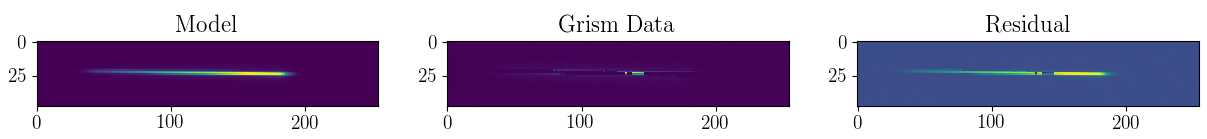
\includegraphics[width=1\textwidth]{images/ex_mod_res.png}\\
   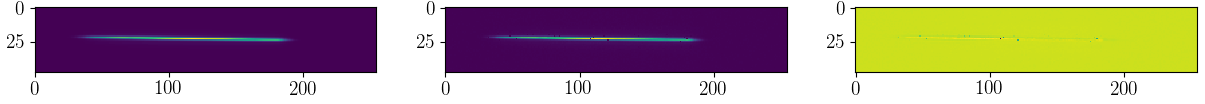
\includegraphics[width=1\textwidth]{images/better_mod_res.png}
    
\caption{\textit{Top: Model, grism data, and residual subtraction of a first order grism trace before Data Quality flagging 
    has been reset to exclude grisms. Bottom: Model, grism data, and residual subtraction after the Data Quality flags
    have been fixed. For both images, the model is a \texttt{pysynphot} normalized model from the X-Shooter spectral library, 
    as described in the next section.}}
\label{fig:beam_trace}
\end{figure}
%fig%%%%-------------------------------------------------------%%%%%%

%%%%%%%%%%%%%%%%%%%%%%%%%%%%%%%%%%%%%%%%%%%%%%%%%%%%%%%%%%%%%%%%%%%%%%%%%%%%%%%%%%%%%%%%%%%
%                                   Analysis
%%%%%%%%%%%%%%%%%%%%%%%%%%%%%%%%%%%%%%%%%%%%%%%%%%%%%%%%%%%%%%%%%%%%%%%%%%%%%%%%%%%%%%%%%%%

\section{Analysis}

\subsection{Reference Spectra}

In the absolute flux calibration below, we adopt the flux reference spectra for GD-71 and GD-153 from the Calspec database (xxx Bohlin), using the model spectra to provide sufficient wavelength resolution: \texttt{gd71\_mod\_010.fits} and \texttt{gd153\_mod\_010.fits}, respectively.

\subsection{Flux Ratios for Throughput Profiles}

Once the traces have been corrected and passed a brief (due to high data volume) visual inspection, we extracted 
the flux vs wavelength profile for each grism order within the images. We display the throughput profiles both in comparison
to the model, as well as ratio them to the model spectra, to give a numerical comparison of where the \texttt{grizli} extraction
is less accurate. Figure \ref{fig:ex_pce} shows an example of one of these figures, and the remaining (which were created
for G102 and G141 on each observable grism order for both calibrator stars) are in Appendix A. 

%fig%%%%-------------------------------------------------------%%%%%%
\begin{figure}[h!]
   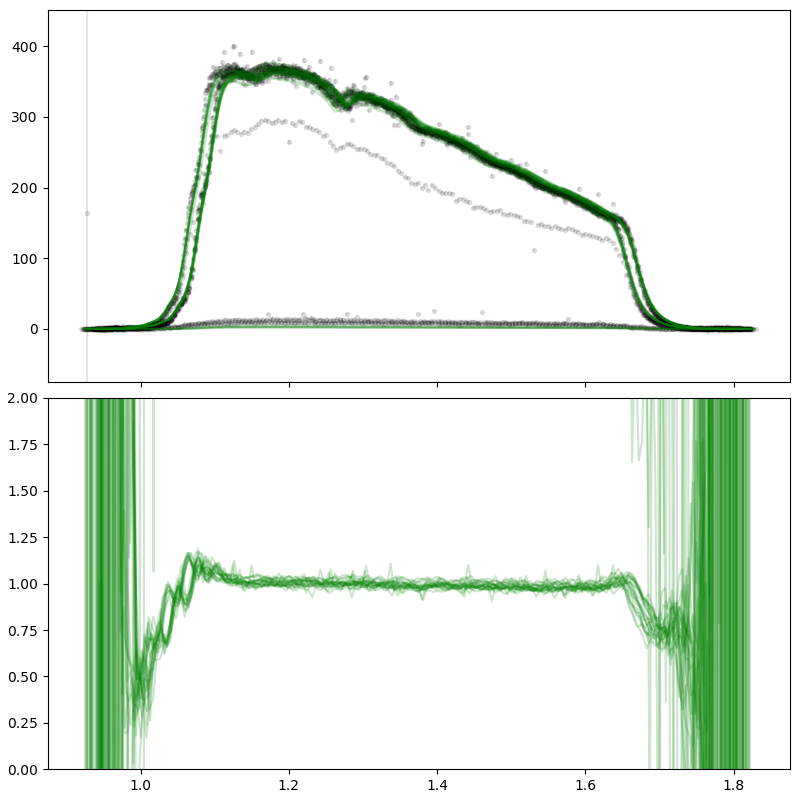
\includegraphics[width=.9\textwidth]{images/ex_pce_ratio.png}
    
\caption{\textit{Top: For the first order beam extracted from each exposure, the black are the extracted data
    and green is the accompanying X-Shooter model. Bottom: This ratio of the model and data shows a close agreement
    except around the edges, where some issue with filter bandpass is to be expected.}}
\label{fig:ex_pce}
\end{figure}
%fig%%%%-------------------------------------------------------%%%%%%
    
\subsection{Sensitivity Curves?} 



%%%%%%%%%%%%%%%%%%%%%%%%%%%%%%%%%%%%%%%%%%%%%%%%%%%%%%%%%%%%%%%%%%%%%%%%%%%%%%%%%%%%%%%%%%%
%                               Results
%%%%%%%%%%%%%%%%%%%%%%%%%%%%%%%%%%%%%%%%%%%%%%%%%%%%%%%%%%%%%%%%%%%%%%%%%%%%%%%%%%%%%%%%%%%

\subsection{Updated Configuration Files}


%%%%%%%%%%%%%%%%%%%%%%%%%%%%%%%%%%%%%%%%%%%%%%%%%%%%%%%%%%%%%%%%%%%%%%%%%%%%%%%%%%%%%%%%%%%
%                                           Acknowledgments 
%%%%%%%%%%%%%%%%%%%%%%%%%%%%%%%%%%%%%%%%%%%%%%%%%%%%%%%%%%%%%%%%%%%%%%%%%%%%%%%%%%%%%%%%%%%
\section{Acknowledgements}
\setlength{\parindent}{0pt}

Thank you to .. for their invaluable comments and feedback on this ISR, as well as the
STScI IT department for helping to make a \texttt{grizli} cookbook available on readthedocs.

%%%%%%%%%%%%%%%%%%%%%%%%%%%%%%%%%%%%%%%%%%%%%%%%%%%%%%%%%%%%%%%%%%%%%%%%%%%%%%%%%%%%%%%%%%%
%                                            Reference List
%%%%%%%%%%%%%%%%%%%%%%%%%%%%%%%%%%%%%%%%%%%%%%%%%%%%%%%%%%%%%%%%%%%%%%%%%%%%%%%%%%%%%%%%%%%
\newpage
\section{References}
\setlength{\parindent}{0pt}

Baggett, S. et al. 2006, Proc. of SPIE, 6265, 626532-2, ``Filters for HST Wide Field Camera 3''

ISR 2016-06: ACS Cycle 24: Here There Be Dragons: Characterization of ACS/WFC Scattered Light Anomalies, B. Porterfield et al. 01 Nov 2016

Lasker, B. et al. 2008, AJ, 136, 735, ``The Second-Generation Guide Star Catalog: Description and Properties''

Skrutskie, M. F. et al. 2006, AJ, 131, 1163, ``The Two Micron All Sky Survey (2MASS)''

The Hubble Space Telescope Wide Field Camera 3 Quicklook Project, Bourque,
Matthew, Bajaj, Varun, Bowers, Ariel, Dulude, Micheal, Durbin, Meredith, Gosmeyer,
Catherine, Gunning, Heather, Khandrika, Harish, Martlin, Catherine, Sunnquist, Ben,
Viana, Alex, ADASS 2016 (proceedings in press)

TIR 2017-01: Aladin Overlay of a Zone of Avoidance for Dragon's Breath, P. R. McCullough 2017 (in prep)



%%%%%%%%%%%%%%%%%%%%%%%%%%%%%%%%%%%%%%%%%%%%%%%%%%%%%%%%%%%%%%%%%%%%%%%%%%%%%%%%%%%%%%%%%%%
%                                            Appendix A
%%%%%%%%%%%%%%%%%%%%%%%%%%%%%%%%%%%%%%%%%%%%%%%%%%%%%%%%%%%%%%%%%%%%%%%%%%%%%%%%%%%%%%%%%%%
\newpage
\section{Appendix A}

Following, we show the model vs data extraction for each filter, source, and grism order combination.


%DEM FIGS!


%%%%%%%%%%%%%%%%%%%%%%%%%%%%%%%%%%%%%%%%%%%%%%%%%%%%%%%%%%%%%%%%%%%%%%%%%%%%%%%%%%%%%%%%%%%
%                                        End of Document
%%%%%%%%%%%%%%%%%%%%%%%%%%%%%%%%%%%%%%%%%%%%%%%%%%%%%%%%%%%%%%%%%%%%%%%%%%%%%%%%%%%%%%%%%%%
\clearpage
\end{document}
